\documentclass[a4paper,10pt]{article}
\usepackage[utf8]{inputenc}

% ----  Useful packages % ---- 
\usepackage{amsmath}
\usepackage{graphicx}
\graphicspath{{images/}}
\usepackage{amsfonts}
\usepackage{amsthm}
\usepackage{amssymb}
\usepackage{makecell}
\usepackage{mathtools}
\usepackage{tikz}
\usepackage{pgfplots}
\usepackage{float}
\usetikzlibrary{arrows.meta}

% ----  Useful packages % ---- 

\usepackage{wrapfig}
\usepackage{caption}
\usepackage{subcaption}
\usepackage{hyperref}
\hypersetup{
	colorlinks,
	citecolor=black,
	filecolor=black,
	linkcolor=black,
	urlcolor=black
}

% ---- Set page size and margins replace ------
\usepackage[letterpaper,top=2cm,bottom=2cm,left=3cm,right=3cm,marginparwidth=1.75cm]{geometry}
% ---- Set page size and margins replace ------

% ------- NOTA ------
\theoremstyle{remark}
\newtheorem{note}{Note}[subsection]
% ------- NOTA ------

% ------- OSSERVAZIONE ------
\theoremstyle{definition}
\newtheorem{observation}{Osservazione}[subsection]
% ------- OSSERVAZIONE ------

% ------- DEFINIZIONE ------
\theoremstyle{plain}
\newtheorem{definition}{Definizione}[subsection]
% ------- DEFINIZIONE ------

% ------- ESEMPIO ------
\theoremstyle{definition}
\newtheorem{example}{Esempio}[subsection]
% ------- ESEMPIO ------

% ------- DIMOSTRAZIONE ------
\theoremstyle{definition}
\newtheorem{demostration}{Dimotrazione}[subsection]
% ------- DIMOSTRAZIONE ------

% ------- TEOREMA ------
\theoremstyle{definition}
\newtheorem{theorem}{Teorema}[subsection]
% ------- TEOREMA ------

% ------- COROLLARIO ------
\theoremstyle{plain}
\newtheorem{corollaries}{Corollario}[theorem]
% ------- COROLLARIO ------

% ------- PROPOSIZIONE ------
\theoremstyle{plain}
\newtheorem{proposition}{Proposizione}[subsection]
% ------- PROPOSIZIONE ------

% ---- Footer and header ---- 
\usepackage{fancyhdr}
\pagestyle{fancy}
\fancyhf{}
\fancyhead[LE,RO]{A.A 2024-2025}
\fancyhead[RE,LO]{Ingegneria del Software}
\fancyfoot[RE,LO]{\rightmark}
\fancyfoot[LE,RO]{\thepage}

\renewcommand{\headrulewidth}{.5pt}
\renewcommand{\footrulewidth}{.5pt}
% ---- Footer and header ---- 

% ----  Language setting ---- 
\usepackage[italian, english]{babel}
% ----  Language setting ---- 

\usepackage{listings}
\usepackage{color}

\definecolor{dkgreen}{rgb}{0,0.6,0}
\definecolor{gray}{rgb}{0.5,0.5,0.5}
\definecolor{mauve}{rgb}{0.58,0,0.82}

\lstset{frame=tb,
	language=C,
	aboveskip=3mm,
	belowskip=3mm,
	showstringspaces=false,
	columns=flexible,
	basicstyle={\small\ttfamily},
	numbers=none,
	numberstyle=\tiny\color{gray},
	keywordstyle=\color{blue},
	commentstyle=\color{dkgreen},
	stringstyle=\color{mauve},
	breaklines=true,
	breakatwhitespace=true,
	tabsize=3
}

\definecolor{lightgray}{rgb}{.9,.9,.9}
\definecolor{darkgray}{rgb}{.4,.4,.4}
\definecolor{purple}{rgb}{0.65, 0.12, 0.82}
\lstdefinelanguage{JavaScript}{
	keywords={break, case, catch, continue, debugger, default, delete, do, else, false, finally, for, function, if, in, instanceof, new, null, return, switch, this, throw, true, try, typeof, var, void, while, with},
	morecomment=[l]{//},
	morecomment=[s]{/*}{*/},
	morestring=[b]',
	morestring=[b]",
	ndkeywords={class, export, boolean, throw, implements, import, this},
	keywordstyle=\color{blue}\bfseries,
	ndkeywordstyle=\color{darkgray}\bfseries,
	identifierstyle=\color{black},
	commentstyle=\color{purple}\ttfamily,
	stringstyle=\color{red}\ttfamily,
	sensitive=true
}

\lstset{
	language=JavaScript,
	extendedchars=true,
	basicstyle=\footnotesize\ttfamily,
	showstringspaces=false,
	showspaces=false,
	tabsize=2,
	breaklines=true,
	showtabs=false,
	captionpos=b
}

\title{\textbf{Ingegneria del software}}
\author{Realizzato da: Ghirardini Filippo}
\date{A.A. 2024-2025}

\begin{document}
	\begin{titlepage} %crea l'enviroment
	\begin{figure}[t] %inserisce le figure
		\centering
\includegraphics[width=0.98\textwidth]{marchio_unipi_pant541.png}
	\end{figure}
	\vspace{20mm}
	
	\begin{Large}
		\begin{center}
			\textbf{Dipartimento di Informatica\\ Corso di Laurea Triennale in Informatica\\}
			\vspace{20mm}
			{\huge{\bf Basi di dati}}\\
			\vspace{5mm}
			{\LARGE{Green City}}\\
			{\large{14 Maggio 2025}}
		\end{center}
	\end{Large}
	
	
	\vspace{36mm}
	\centering{
	\begin{minipage}[t]{0.47\textwidth}
		\centering
		{\large{\bf Autori:}\\ \large{Filippo Ghirardini (654829)}}
	\end{minipage}}
	
\end{titlepage}
	
	\tableofcontents
	\newpage
	\maketitle
	\begin{center}
		\vspace{-20pt}
		\rule{11cm}{.1pt} 
	\end{center}
	% !TeX spellcheck = it_IT
\newpage
\section{Descrizione del dominio}
Un \textbf{concorso} è organizzato da uno o più \textbf{organizzatori}, che devono definire la durata del concorso in giorni, la scadenza per la sottomissione delle opere, la scadenza per la valutazione, il numero massimo di opere che possono essere presentate e la durata massima di ogni opera in minuti. Ogni concorso avrà dei \textbf{generi} consentiti (caratterizzati da un nome e descrizione), delle \textbf{lingue} accettate e dei criteri di partecipazione.\\

Ad ogni concorso un \textbf{regista} (che non può essere l'organizzatore) può presentare dei \textbf{cortometraggi} (fino al massimo indicato dagli organizzatori). Ogni cortometraggio è caratterizzato da un nome, la lingua, il genere, la durata in minuti e una trama.\\

Per ogni concorso gli organizzatori nominano dei \textbf{giudici} che compongono il comitato di valutazione. Ogni cortometraggio \textbf{partecipante} è assegnato a tre giudici, ognuno dei quali uno o più cortometraggi ma tutti di registi diversi. Ogni giudice può nominare un \textbf{giudice esterno} per ogni concorso per la valutazione di uno o più cortometraggi.\\

La valutazione avviene tramite una \textbf{recensione} scritta da un giudice relativamente ad una \textbf{partecipazione} di un cortometraggio, e contiene un punteggio da 0 a 5, un commento generale e una nota riservata.\\

Giudici, organizzatori e registi sono \textbf{utenti} del sistema con nome, cognome, codice fiscale ed email (usata per gli inviti dei giudici).

\newpage
\section{Schema concettuale}
\begin{center}
	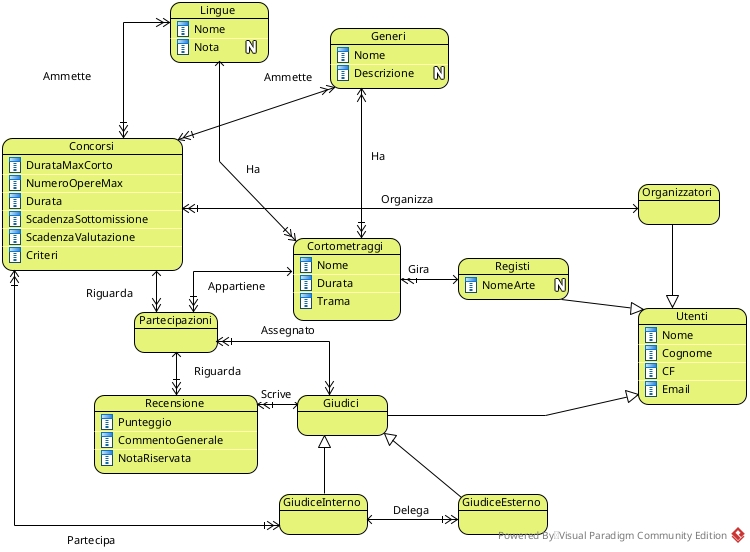
\includegraphics[scale=.5]{ERD_ConCorto.jpg}
\end{center}

\begin{note}
	Al momento della delega da parte di un \textbf{Giudice interno} di un \textbf{Giudice esterno}, quest'ultimo viene inserito nel database e viene assegnato alla valutazione di una determinata \textbf{partecipazione} scelta dal delegante.
\end{note}

\begin{note}
	Al momento dell'inserimento della \textbf{partecipazione} di un \textbf{cortometraggio} ad un \textbf{concorso}, vanno controllati i limiti imposti dall'\textbf{organizzatore} (\textit{DurataMaxCorto}, \textit{NumeroOpereMax}, lingue e generi accettati).
\end{note}

\subsection{Vincoli}
\subsubsection{Interrelazionali}
I vincoli interrelazionali sono:
\begin{itemize}
	\item Un giudice non può giudicare più di un cortometraggio per regista
	\item Un cortometraggio ha 3 giudici assegnati
	\item Un giudice può delegare al più un esterno per ogni concorso
	\item Un organizzatore non può partecipare come regista ad un concorso che organizza
	\item Un giudice può scrivere una sola recensione per cortometraggio per ogni concorso
	\item Se un giudice ha delegato la valutazione non può scrivere la recensione per il cortometraggio che ha delegato
\end{itemize}
\subsubsection{Intrarelazionali}
I vincoli intrarelazionali sono:
\begin{itemize}
	\item \textbf{Generi}: \textit{Descrizione} è NULLABLE
	\item \textbf{Lingue}: \textit{Nota} è NULLABLE
	\item \textbf{Concorsi}: \textit{DurataMaxCorto} $> 0$, \textit{NumeroOpereMax} $>0$, \textit{Durata} $>0$, \textit{ScadenzaSottomissione} $<$ \textit{ScadenzaValutazione}
	\item \textbf{Cortometraggi}: \textit{Durata} $>0$
	\item \textbf{Recensione}: $0\leq$\textit{Punteggio} $\leq 5$
	\item \textbf{Utenti}: \textit{Email} deve rispettare la seguente REGEX
	\begin{lstlisting}[language=Javascript]
		/^[\w-\.]+@([\w-]+\.)+[\w-]{2,4}$/g
	\end{lstlisting}
	\textit{CF} deve rispettare la seguente REGEX
	\begin{lstlisting}[language=Javascript]
		/^(?:[A-Z][AEIOU][AEIOUX]|[AEIOU]X{2}|[B-DF-HJ-NP-TV-Z]{2}[A-Z]){2}(?:[\dLMNP-V]{2}
		(?:[A-EHLMPR-T](?:[04LQ][1-9MNP-V]|[15MR][\dLMNP-V]|[26NS][0-8LMNP-U])|[DHPS]
		[37PT][0L]|[ACELMRT][37PT][01LM]|[AC-EHLMPR-T][26NS][9V])|(?:[02468LNQSU][048LQU]
		|[13579MPRTV][26NS])B[26NS][9V])(?:[A-MZ][1-9MNP-V][\dLMNP-V]{2}|[A-M][0L]
		(?:[1-9MNP-V][\dLMNP-V]|[0L][1-9MNP-V]))[A-Z]$/i
	\end{lstlisting}
	\item \textbf{Registi}: \textit{NomeArte} è NULLABLE
\end{itemize}
Dove non specificato, l'attributo è NON NULLABLE.

\newpage
\section{Schema logico relazionale}
\begin{center}
	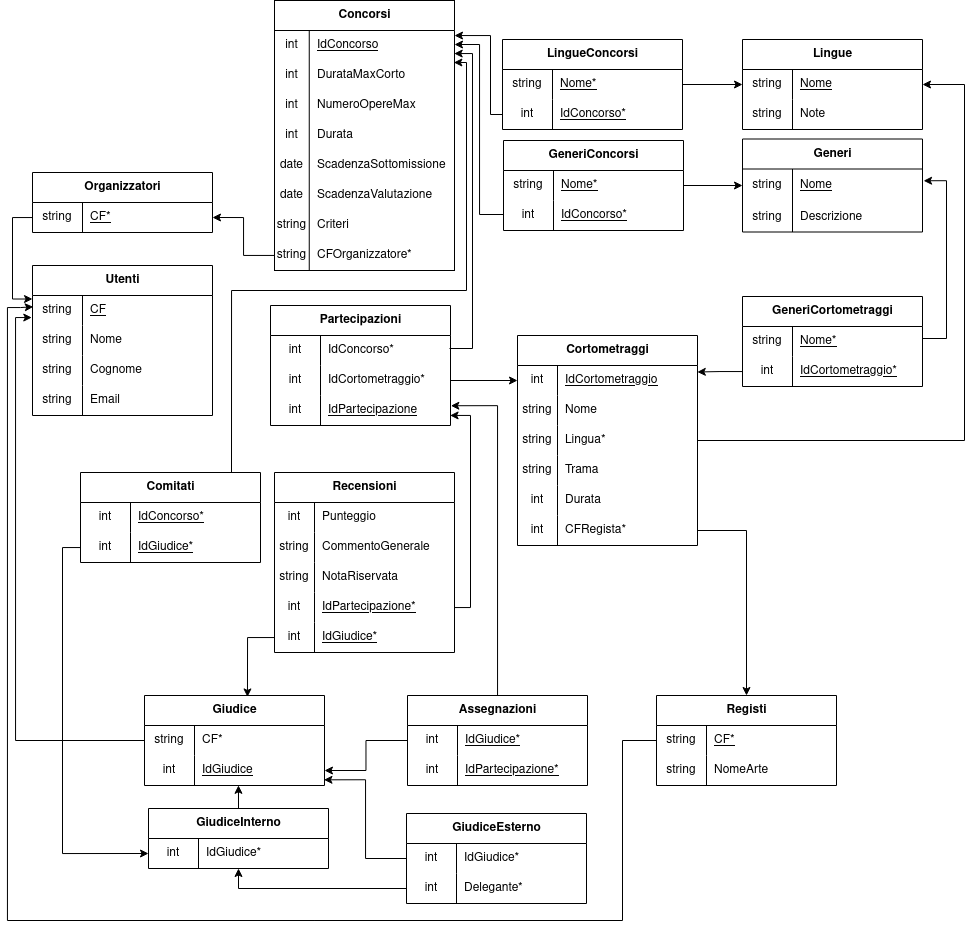
\includegraphics[scale=0.45]{BD0525_logico}
\end{center}

\subsection{Dipendenze funzionali}
Tutte le relazioni $R$ con attributi $A_1, \ldots, A_n$ chiave $K \notin A_1, \ldots, A_n$ hanno una sola dipendenza funzionale del tipo $K \to A_1, \ldots, A_n$.

\subsection{BCNF}
Tutte le relazioni sono in BCNF.

\newpage
\section{Interrogazioni in SQL}
Di seguito le sei interrogazioni richieste:
\begin{enumerate}
	\item[a.] Trova i nomi e le email degli utenti che sono registi e hanno diretto un cortometraggio di durata superiore a 25 minuti.
	\begin{lstlisting}[language=SQL]
		SELECT U.Nome, U.Email
		FROM Utenti U
		JOIN Registi R ON U.CF = R.CF
		JOIN Cortometraggi C ON R.CF = C.CFRegista
		WHERE C.Durata > 25;
	\end{lstlisting}
	\item[b.] Trova i concorsi con più di due lingue ammesse e con una durata massima inferiore a 120 giorni ordinati per numero di lingue in ordine decrescente.
	\begin{lstlisting}[language=SQL]
		SELECT C.IdConcorso, C.Durata, COUNT(L.Nome) AS NumeroLingue
		FROM Concorsi C
		JOIN LingueConcorsi LC ON C.IdConcorso = LC.IdConcorso
		JOIN Lingue L ON L.Nome = LC.Nome
		WHERE C.Durata < 120
		GROUP BY C.IdConcorso, C.Durata
		HAVING COUNT(L.Nome) > 2
		ORDER BY NumeroLingue DESC;
	\end{lstlisting} 
	\item[c.] Trova i generi di cortometraggi lunghi almeno 20 minuti che hanno una durata media superiore a 22 minuti, raggruppati per genere.
	\begin{lstlisting}[language=SQL]
		SELECT G.Nome, AVG(C.Durata) AS DurataMedia
		FROM GeneriCortometraggi GC
		JOIN Generi G ON G.Nome = GC.Nome
		JOIN Cortometraggi C ON C.IdCortometraggio = GC.IdCortometraggio
		WHERE C.Durata > 20
		GROUP BY G.Nome
		HAVING AVG(C.Durata) > 22;
	\end{lstlisting} 
	\item[d.] Trova i nomi dei cortometraggi che hanno almeno una recensione con punteggio superiore a 2.
	\begin{lstlisting}[language=SQL]
		SELECT C.Nome
		FROM Cortometraggi C
		WHERE EXISTS (
			SELECT *
			FROM Recensioni R
			JOIN Partecipazioni P ON R.IdPartecipazione = P.IdPartecipazione
			WHERE P.IdCortometraggio = C.IdCortometraggio AND R.Punteggio > 2
		);
	\end{lstlisting} 
	\item[e.] Trova i nomi dei concorsi in cui tutti i cortometraggi partecipanti hanno una durata inferiore a 30 minuti.
	\begin{lstlisting}[language=SQL]
		SELECT C.IdConcorso
		FROM Concorsi C
		WHERE NOT EXISTS (
		SELECT *
			FROM Partecipazioni P
			JOIN Cortometraggi CM ON P.IdCortometraggio = CM.IdCortometraggio
			WHERE P.IdConcorso = C.IdConcorso AND CM.Durata >= 30
		);
	\end{lstlisting}
	\newpage
	\item[f.] Trova i giudici che hanno assegnato un punteggio superiore alla media dei punteggi di tutti i giudici.
	\begin{lstlisting}[language=SQL]
		SELECT G.IdGiudice, G.CF
		FROM Giudici G
		WHERE EXISTS (
			SELECT *
			FROM Recensioni R
			WHERE R.IdGiudice = G.IdGiudice AND R.Punteggio > (
				SELECT AVG(Punteggio) 
				FROM Recensioni
			)
		);
	\end{lstlisting} 
\end{enumerate}

\newpage
\section{Piani di accesso}
\begin{enumerate}
	\item[I.] Piani di accesso \textbf{logico}
	\begin{figure}[!h]
		\centering
		\begin{minipage}{\textwidth}
			\centering
			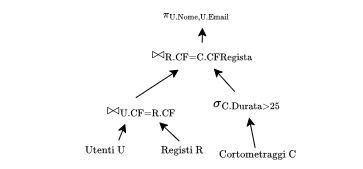
\includegraphics[scale=0.7]{1a.png}
			\captionof{figure}{Query \textit{a}}
		\end{minipage}
		\begin{minipage}{\textwidth}
			\centering
			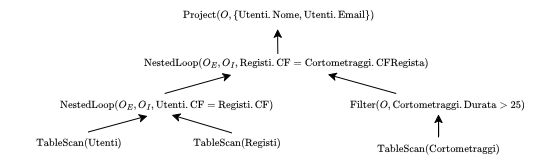
\includegraphics[scale=0.7]{1b.png}
			\captionof{figure}{Query \textit{b}}
		\end{minipage}
		\begin{minipage}{\textwidth}
			\centering
			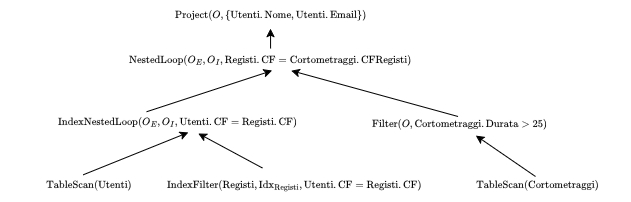
\includegraphics[scale=0.65]{1c.png}
			\captionof{figure}{Query \textit{c}}
		\end{minipage}
	\end{figure}
	
	\newpage
	\item[II.] Piani di accesso \textbf{fisico} senza uso di indici
	\begin{figure}[!h]
		\centering
		\begin{minipage}{\textwidth}
			\centering
			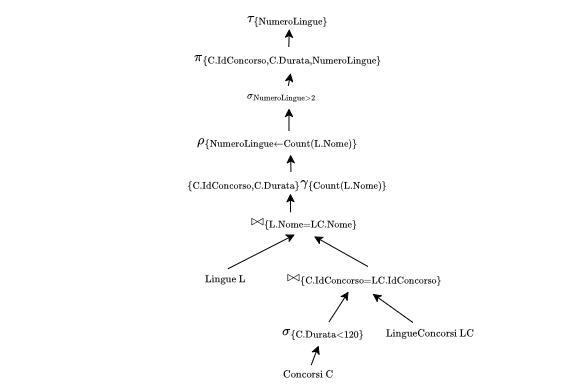
\includegraphics[scale=0.7]{2a.png}
			\captionof{figure}{Query \textit{a}}
		\end{minipage}\\
		\begin{minipage}{\textwidth}
			\centering
			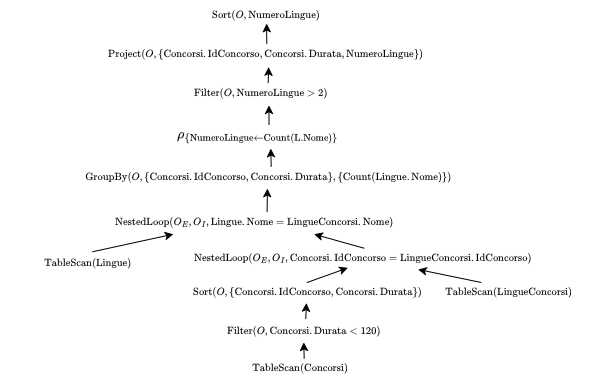
\includegraphics[scale=0.7]{2b.png}
			\captionof{figure}{Query \textit{b}}
		\end{minipage}
	\end{figure}
	\begin{figure}[!h]
		\centering
		\begin{minipage}{\textwidth}
			\centering
			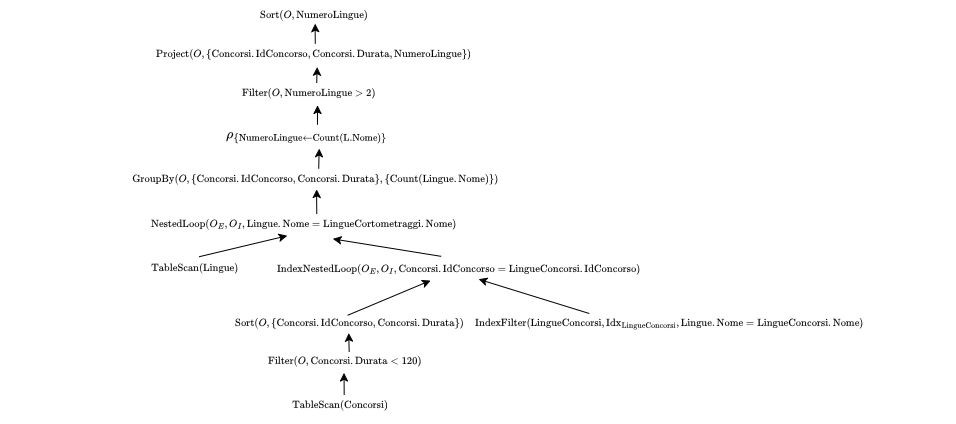
\includegraphics[scale=0.55]{2c.png}
			\captionof{figure}{Query \textit{c}}
		\end{minipage}
	\end{figure}
	
	\newpage
	\item[III.] Piani di accesso \textbf{fisico} con uso di indici
	\begin{figure}[!h]
		\centering
		\begin{minipage}{\textwidth}
			\centering
			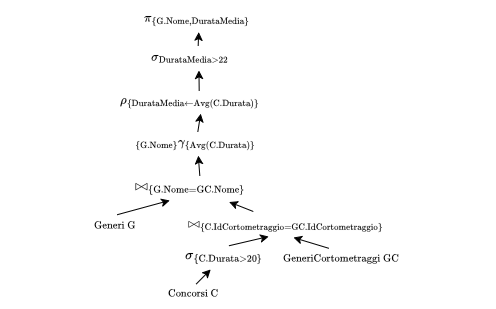
\includegraphics[scale=0.7]{3a.png}
			\captionof{figure}{Query \textit{a}}
		\end{minipage}\\
	\end{figure}
	\begin{figure}[!h]
		\centering
		\begin{minipage}{\textwidth}
			\centering
			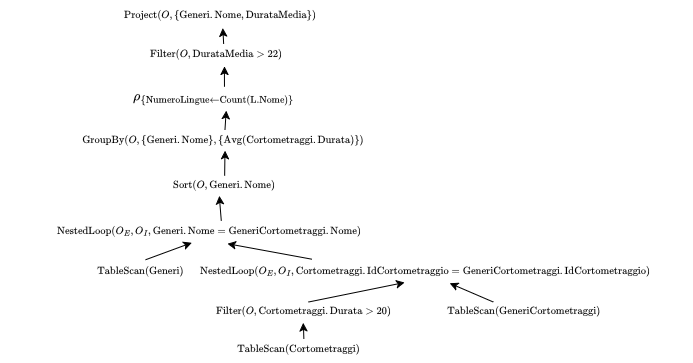
\includegraphics[scale=0.7]{3b.png}
			\captionof{figure}{Query \textit{b}}
		\end{minipage} \hspace{50pt}
		\begin{minipage}{\textwidth}
			\centering
			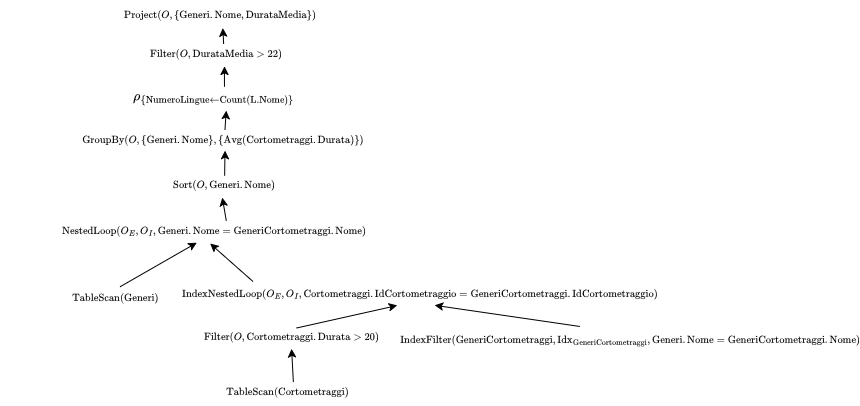
\includegraphics[scale=0.45]{3c.png}
			\captionof{figure}{Query \textit{c}}
		\end{minipage}
	\end{figure}
\end{enumerate}
	\input{softwareprocesses}
	\input{requisiti}
	\input{UML}
	% !TeX spellcheck = it_IT
\newpage
\section{Progettazione}
La fase di progettazione è tra quella della specifica (cosa fare) e quella della programmazione. Come risultato produce un'\textbf{architettura} che descrive \textbf{come} fare.\\
Possono esserci due livelli di astrazione:
\begin{itemize}
	\item \textbf{Architetturale}: si scompone un sistema in più sottosistemi, ne si identificano e specificano le parti e le interconnessioni
	\item Di \textbf{dettaglio}: indica come la specifica di ogni parte sarà realizzata
\end{itemize}

\begin{definition}[Architettura software]
	L’architettura di un sistema software è la \textbf{struttura} del sistema, costituita dalle parti del sistema, dalle \textbf{relazioni} tra le parti e dalle loro proprietà visibili.
\end{definition}

\begin{definition}[Stile architetturale]
	Uno stile architetturale caratterizza una famiglia di architetture con caratteristiche simili (e.g. client-server, microservizi). Le funzionalità e le interazioni tra i componenti spesso seguono degli standard.
\end{definition}

Un'architettura si sviluppa in diverse \textbf{viste} e \textbf{stili}.

\begin{center}
	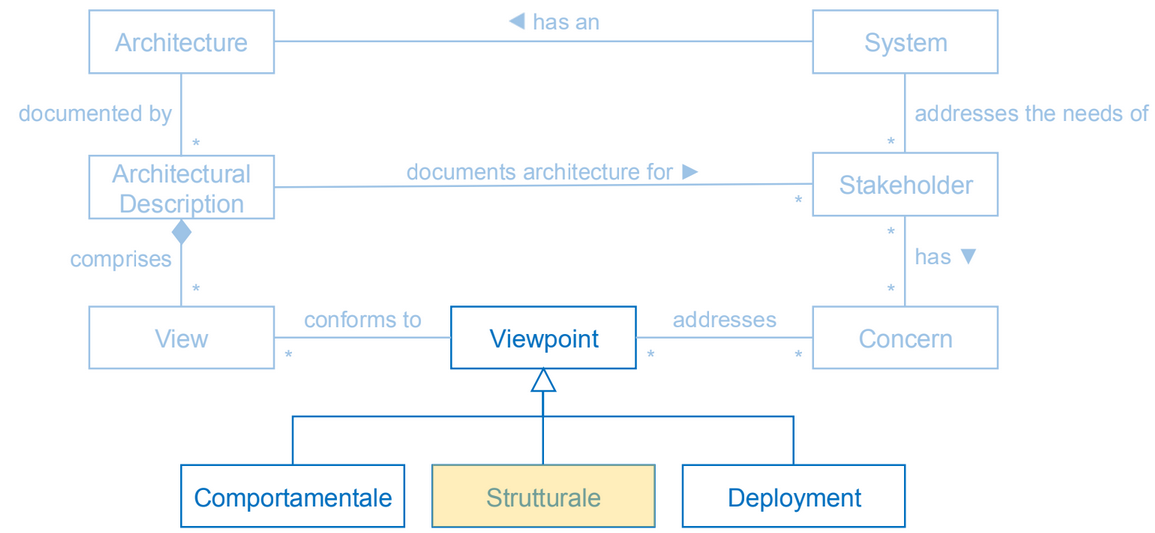
\includegraphics[scale=0.3]{progettazione}
\end{center}

\subsection{Vista comportamentale}
Anche detta \textbf{component-and-connector}, descrive un sistema software come \textbf{composizione di componenti}, compreso di:
\begin{itemize}
	\item \textbf{Interfacce} dei componenti
	\item Caratteristiche dei \textbf{connettori}
	\item Struttura del sistema in esecuzione (flusso dei dati, parallelismo, replicazioni, etc..)
\end{itemize}
Questa vista permette l'analisi delle \textbf{caratteristiche di qualità} a tempo di esecuzione (prestazioni, affidabilità, etc..) e di documentare lo \textbf{stile} dell'architettura.

\subsubsection{Componente}
Una componente software è un'unità concettuale di decomposizione del sistema a tempo di esecuzione. Incapsula un insieme di \textbf{funzionalità} e/o \textbf{dati}, restringendone l'accesso tramite delle \textbf{interfacce}.
\begin{definition}[Componente]
	Una componente software è un'unità di software \textbf{indipendente} e \textbf{riutilizzabile}.
\end{definition}

\begin{definition}[Sistema software]
	Un sistema software è una composizione di componenti software basata sulla connessione di più componenti e realizzata con interfacce dei componenti e connettori,
\end{definition}

\noindent In UML un componente è un \textbf{classificatore} e si compone di:
\paragraph{Porti} I porti ne identificano i punti di interazione. Può essercene più di uno, possono fornire o richiedere una o più \textit{interfacce} e possono avere \textit{nomi} e \textit{molteplicità}.
\begin{center}
	\includegraphics[scale=0.3]{component.png}
\end{center}
I porti possono avere la specifica delle interfacce in due modi:
\begin{itemize}
	\item \textbf{Sintetica}: si indica solo quando è \textit{richiesta} (forchetta) o offerta (\textit{lollipop})
	\begin{center}
		\includegraphics[scale=0.2]{interfaccia_sintetica.png}
	\end{center}
	\item \textbf{Estesa}: si specifica per esteso le operazioni richieste ed offerte
	\begin{center}
		\includegraphics[scale=0.2]{interfaccia_estesa.png}
	\end{center}
\end{itemize}

\paragraph{Connettori}
I connettori sono \textbf{canali di interazione} tra i porti di componenti. Non hanno un descrittore specifico e vengono rappresentati come associazioni. Per dare più informazioni si indica lo \textbf{stile} della connessione o con uno \textbf{stereotipo} o indicando i \textbf{ruoli}.

\begin{center}
	\includegraphics[scale=0.3]{connettori.png}
\end{center}

\subsubsection{Stili}
In questo tipo di vista uno stile architetturale è caratterizzato dalle \textbf{caratteristiche generali} delle componenti e dalle loro \textbf{interazioni} (quindi \textit{porti} e \textit{connettori}).

\paragraph{Pipes \& filters} Questo stile consiste in un flusso di elaborazione di dati che viaggiano lungo le \textbf{pipe} e sono processati dai \textbf{filter}. In particolare i \textit{filter} sono i \textbf{componenti} che trasformano i flussi di dati mentre le \textit{pipe} sono i \textbf{connettori} che fungono da canale di comunicazione unidirezionale bufferizzato che preserva l'ordine di ingresso.
\begin{center}
	\includegraphics[scale=0.3]{pipes_filters.png}
\end{center}

\paragraph{Client-server} Questo stile prevede due componenti che possono essere su macchine diverse. Il \textbf{server} offre il servizio, aspetta le richieste dati ad un porto e può servirne su di esso più alla volta. Il \textbf{client} invia richieste al server e attende una risposta.
\begin{center}
	\includegraphics[scale=0.3]{client-server.png}
\end{center}
Il server in particolare prevede un \textbf{RequestListener} in attesa di richieste e un \textbf{RequestHandler} per ognuna di esse. Quest'ultimo elabora le richieste e:
\begin{itemize}
	\item Se \textbf{stateless} le gestisce ognuna in maniera indipendente
	\item Se \textbf{stateful} consente richieste \textit{composite} che consistono in più richieste \textit{atomiche}, mantenendo un record di esse \textbf{sessione}
\end{itemize}

\paragraph{Master-slave}
Questo stile è una variazione di \textit{client-server} in cui c'è solamente un servente (\textbf{slave}) e un cliente (\textbf{master})

\paragraph{Peer to Peer} Questo stile è una variazione di \textit{client-server} dove tutti i componenti sono sia client che server e avviene uno scambio di servizi alla pari.
\begin{center}
	\includegraphics[scale=0.6]{p2p.png}
\end{center}

\paragraph{Publish-Subscribe} In questo stile i componenti interagiscono in modo \textbf{event-based}. Abbiamo tre tipi di componenti:
\begin{itemize}
	\item \textbf{Publisher}: produce classi di eventi
	\item \textbf{Subscriber}: si iscrive alle classi rilevanti
	\item \textbf{Broker}: smista gli eventi pubblicati
\end{itemize}
Un componente può essere sia \textit{publisher} che \textit{subscriber}. Tra di loro comunicano tramite il \textit{broker}.I publisher non sanno quanti/quali subscriber ci siano e viceversa, garantendo \textbf{scalabilità}.
Questo stile può funzionare in due modi:
\begin{itemize}
	\item \textbf{Push}: il broker invia attivamente i messaggi ai subscriber, controllandone la frequenza
	\item \textbf{Pull}: è il subscriber che manualmente recupera i messaggi dal broker. Migliora la scalabilità e la flessibilità dato che servono meno broker.
\end{itemize}

\begin{figure}[!h]
	\centering
	\begin{minipage}[b]{0.5\textwidth}
		\includegraphics[width=\textwidth]{pub-sub.png}
	\end{minipage}
	\hfill
	\begin{minipage}[b]{0.4\textwidth}
		\includegraphics[width=\textwidth]{pub_sub_full.png}
	\end{minipage}
\end{figure}

\paragraph{Process coordinator}
Un componente funge da \textbf{process coordinator} mentre gli altri sono passivi e non conoscono il loro ruolo nel processo ma si limitano a contribuire. Il \textit{coordinator} conosce la sequenza di passi necessaria, invoca le funzionalità richieste e fornisce una risposta.

\paragraph{Model-View-Controller/Publisher}
Questo stile si basa su tre elementi:
\begin{itemize}
	\item \textbf{Model}: nucleo funzionale che implementa la business logic dell'applicazione e ne rappresenta i dati su cui essa lavora
	\item \textbf{View}: presentazione del model all'utente, possono essercene diverse
	\item \textbf{Controller}: controlla l'input dell'utente e lo traduce in operazioni da eseguire su \textit{model} oppure \textbf{presenter} in alternativa
\end{itemize}
\begin{figure}[!h]
	\centering
	\begin{minipage}[b]{0.4\textwidth}
		\includegraphics[width=\textwidth]{model_view_controller.png}
		\caption*{Controller}
	\end{minipage}
	\hspace{10pt}
	\begin{minipage}[b]{0.4\textwidth}
		\includegraphics[width=\textwidth]{model_view_presenter.png}
		\caption*{Presenter}
	\end{minipage}
\end{figure}

\subsection{Vista strutturale}
Descrive la struttura di un sistema software come insieme di \textbf{unità di realizzazione}, ovvero di codice. Permette di analizzare le \textbf{dipendenze}, progettare i \textbf{test} e valutare la \textbf{portabilità}.\\
La vista strutturale in UML include:
\begin{itemize}
	\item \textbf{Classi} con specifica delle \textit{operazioni} più dettagliata rispetto alla descrizione del dominio
	\item \textbf{Package}
\end{itemize}

\subsubsection{Decomposizione}
\begin{wrapfigure}[7]{r}{5cm}
	\vspace{-1.2cm}
	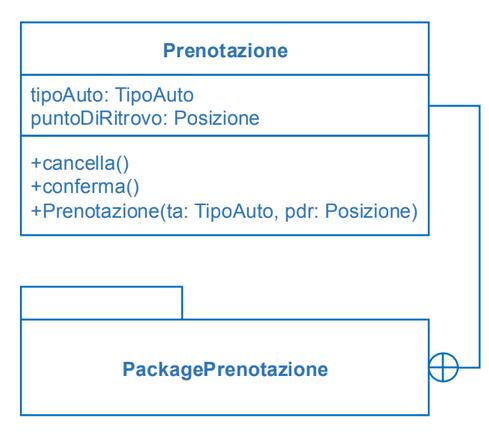
\includegraphics[width=5cm]{decomposizione}
\end{wrapfigure}
Una classe può far parte (essere contenuta in) un package, che a sua volta può far parte di uno più grande. La decomposizione può essere fatta per \textbf{apprendimento} del sistema o per l'\textbf{allocazione del lavoro} e può seguire tre criteri:
\begin{itemize}
	\item Incapsulamento per \textbf{modificabilità}
	\item Supporto alle scelte \textbf{costruisci}/\textbf{compra}
	\item Moduli comuni in \textbf{linee di prodotto}
\end{itemize}

\begin{note}
	La relazione "parte di" si può rappresentare anche con l'inclusione grafica in un package.
\end{note}

\newpage

\subsubsection{Uso}
Un modulo A può usarne un altro B per soddisfare i suoi requisiti. Questo permette di pianificare uno sviluppo incrementale e creare test di unità ed integrazione. Sono permessi i cicli anche se pericolosi.

\begin{center}
	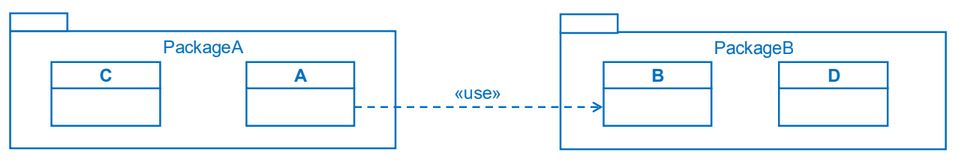
\includegraphics[scale=0.4]{uso}
\end{center}

\subsubsection{Strati}
\begin{wrapfigure}[10]{r}{3cm}
	\vspace{-1cm}
	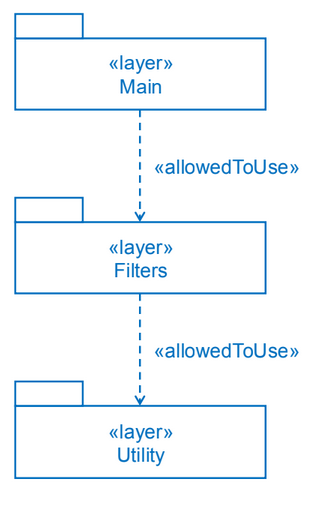
\includegraphics[width=3cm]{strati}
\end{wrapfigure}
Nella vista strutturale a strati ogni elemento (\textbf{strato}) è un insieme coeso di moduli a volte raggruppati in segmenti, il quale offre un'interfaccia pubblica per i suoi servizi. La relazione \textit{allowedToUse} è un caso particolare di quella di uso ed è \textbf{antisimmetrica} e \textbf{non implicitamente transitiva}.\\
Questa vista favorisce modificabilità, portabilità e controllo della complessità.

\subsubsection{Generalizzazione}
In questa vista gli elementi sono i \textbf{moduli} (classi o packages) che hanno una relazione di generalizzazione tra di loro. Permette di rappresentare relazioni di sotto tipo tra classi e la relazione tra un framework\footnote{Collezione di classi, anche astratte, con relazioni d'uso tra loro.} e una sua specializzazione nel caso dei package.

\subsection{Vista di deployment}
Descrive l'allocazione del software su ambienti di esecuzione e permette di valutarne \textbf{prestazioni} e \textbf{affidabilità}. Contiene:
\begin{itemize}
	\item \textbf{Artefatti} prodotti da un processo di sviluppo software o dal funzionamento di un sistema, rappresentati dallo stereotipo \textit{$<<$artifact$>>$}
	\item \textbf{Ambienti di esecuzione} o nodi hardware, rappresentati come \textit{parallelepipedi}
\end{itemize}
Questi elementi possono avere due tipi di relazioni:
\begin{itemize}
	\item \textbf{Dislocazione} di artefatti negli ambienti, rappresentata con il \textit{contenimento}
	\item \textbf{Interconnessione} tra gli ambienti di esecuzione, rappresentate con relazioni stereotipate
\end{itemize}
\begin{center}
	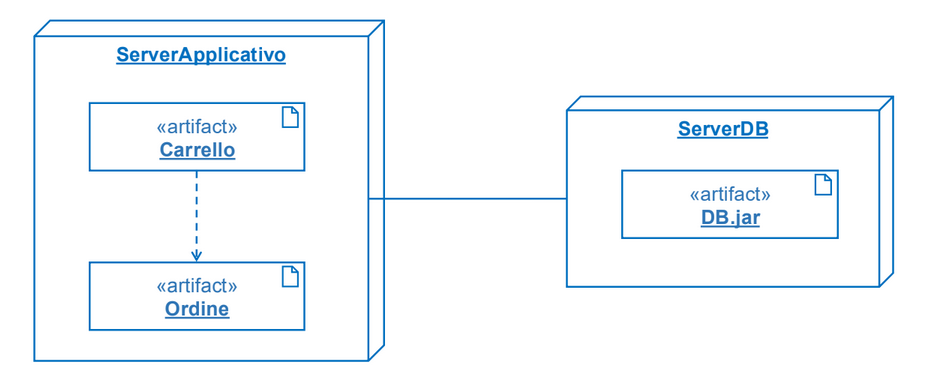
\includegraphics[scale=.4]{deployment}
\end{center}

\subsection{Vista ibrida}
La vista ibrida si compone di quella comportamentale e di quella di deployment su di un'applicazione 3-tier.
\begin{center}
	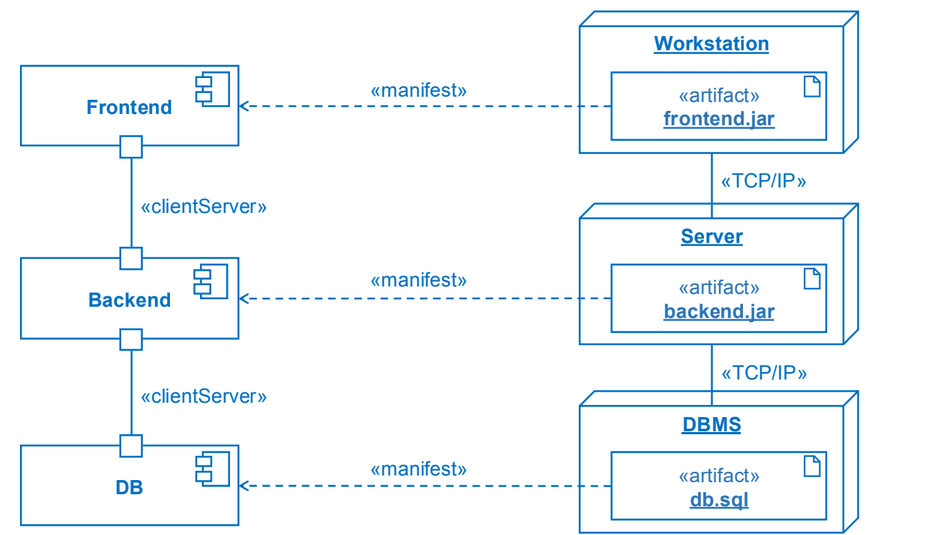
\includegraphics[scale=.4]{ibride}
\end{center}

\subsection{Altri esempi}
\subsubsection{Architettura a livelli}
\begin{wrapfigure}[9]{r}{6cm}
	\vspace{-1cm}
	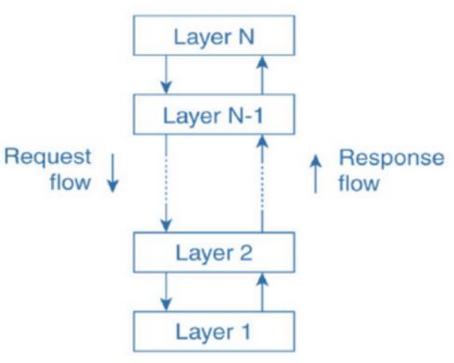
\includegraphics[width=6cm]{livelli}
\end{wrapfigure}
I componenti sono organizzati in livelli (layer) dove uno a livello $i$ può invocarne uno del livello sottostante $i-1$. Le richieste scendono lungo la gerarchia mentre le risposte salgono.

\subsubsection{Architettura multi-livello}
In questa architettura avviene un mapping tra livelli logici (layer) e fisici (tier). Può avere da $1$ ad $N$ livelli, dove all'aumentare di questi si guadagna in \textbf{flessibilità}, \textbf{funzionalità} e possibilità di \textbf{distribuzione} ma si introducono problemi di \textbf{prestazione}. \\
Dal punto di vista fisico, l'architettura può essere:
\begin{itemize}
	\item \textbf{1-tier}: mainframe e terminale
	\item \textbf{2-tier}: macchina client e singolo server
	\item \textbf{3-tier}: ciascun livello su una macchina separate
\end{itemize}
\begin{center}
	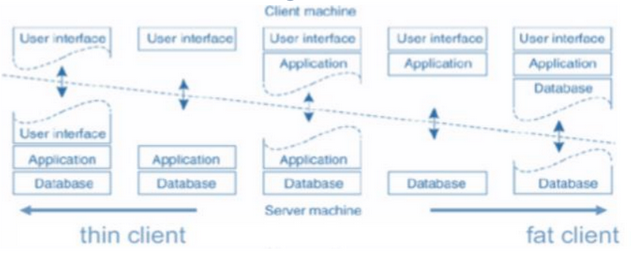
\includegraphics[scale=.4]{multiliv}
\end{center}
	% !TeX spellcheck = it_IT
\newpage
\section{Diagrammi di sequenza}
\begin{wrapfigure}[10]{r}{5cm}
	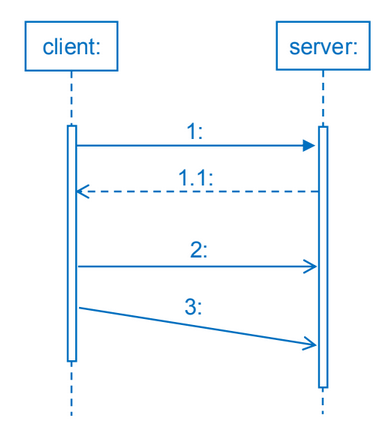
\includegraphics[width=5cm]{diagseq}
\end{wrapfigure}
I diagrammi di sequenza descrivono le \textbf{interazioni} tra oggetti riorganizzandole in una sequenza temporale. Nella fase di \textit{analisi} dei casi d'uso formalizzano la sequenza principale  degli eventi mentre in fase di \textit{progettazione} illustrano come l'architettura realizza i requisiti.\\

In UML per ogni partecipante viene disegnata una \textbf{linea di vita} che può essere tratteggiata quando l'oggetto è inattivo e doppia-continua quando è attivo. Per rappresentare le \textbf{interazioni} vengono usate frecce, che possono essere:
\begin{itemize}
	\item \textbf{Sincrone}
	\item \textbf{Ritorno}
	\item \textbf{Asincrone}
	\item Asincrone con \textbf{consumo di tempo}
\end{itemize}

\subsection{Etichette}
È possibile mettere etichette ai messaggi:
\begin{itemize}
	\item $n$ è il numero del messaggio nella sequenza
	\item \textbf{attr} è l'attributo a cui assegnare il valore restituito
	\item \textbf{name} identifica e descrive il messaggio
	\item \textbf{arg} sono i parametri
	\item \textbf{value} rappresenta il valore restituito
\end{itemize}
\begin{center}
	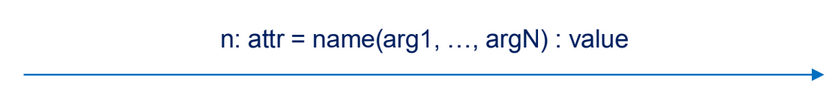
\includegraphics[scale=.4]{etichette}
\end{center}

\subsection{Creazione e distruzione}
Un oggetto può crearne o eliminarne un altro attraverso lo scambio di messaggi.
\begin{center}
	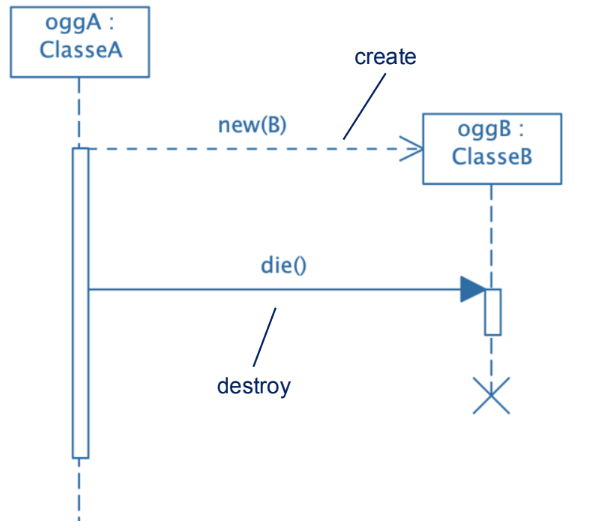
\includegraphics[scale=0.4]{creazdist}
\end{center}

\subsection{Frame}
\subsubsection{Condizionale}
È identificato dalla parola \textbf{alt}. I subframe possono essere etichettati con guardie:
\begin{itemize}
	\item Se non c'è la guardia, è \textit{true}
	\item Se ci sono più guardie vere è una situazione di non determinismo
	\item Se ci sono tutte le guardie false, si salta il frame
\end{itemize}
\begin{center}
	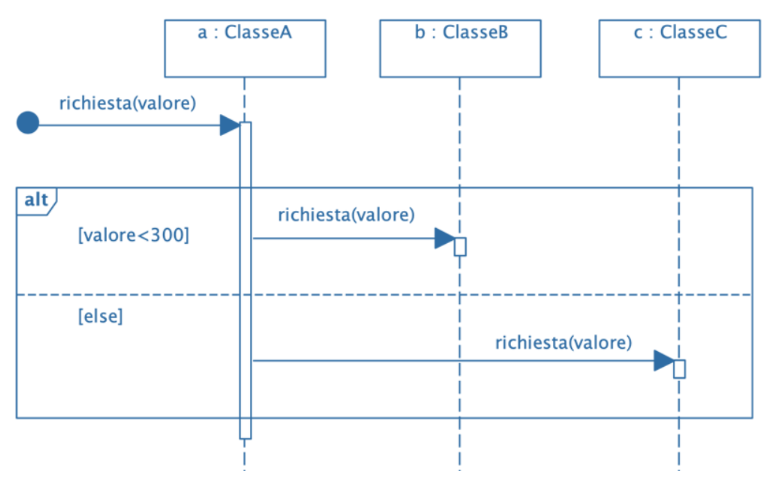
\includegraphics[scale=.3]{condiz}
\end{center}

\subsubsection{Opzionale}
Il frame opzionale è identificato dalla parola chiave \textbf{opt} e le interazioni sono eseguite solo se la guardia è vera, altrimenti il frame viene saltato.
\begin{center}
	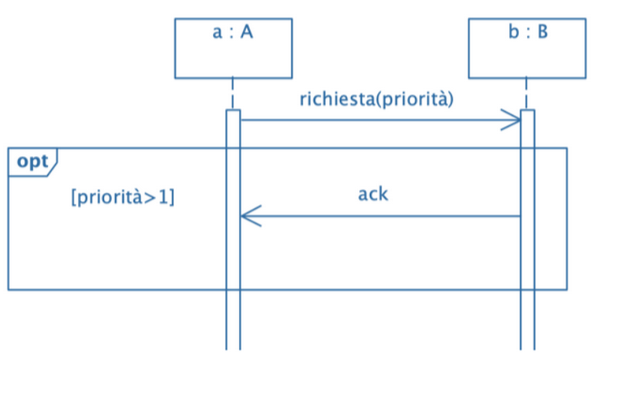
\includegraphics[scale=.3]{opz}
\end{center}

\subsubsection{Iterativo}
Questo frame ripete il suo contenuto da \textit{min} a \textit{max}, \textbf{loop(min, max)} e finché la \textbf{condizione} è vera. Quindi le implementazioni dei classici cicli sono:
\begin{itemize}
	\item \textbf{while}: loop(0,*)[guardia] e loop[guardia]
	\item \textbf{do-while}: loop(1,*)[guardia]
	\item \textbf{for}: loop(n,n) e loop(n)
\end{itemize}
\begin{center}
	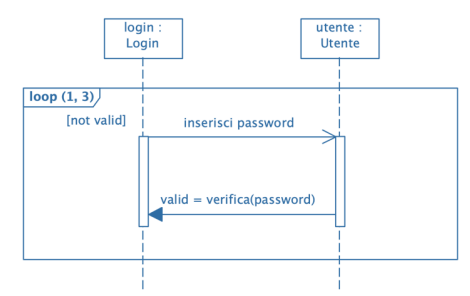
\includegraphics[scale=.4]{cicli}
\end{center}

\subsubsection{Parallelo}
Identificato da \textbf{par}, indica che le interazioni nei sotto-frammenti sono eseguite in parallelo con una semantica ad interleaving.

\begin{center}
	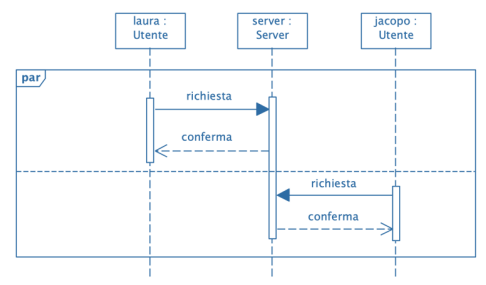
\includegraphics[scale=.5]{parall}
\end{center}

\subsection{Inclusione}
È possibile includere un'interazione definita altrove tramite \textbf{ref}.
\begin{center}
	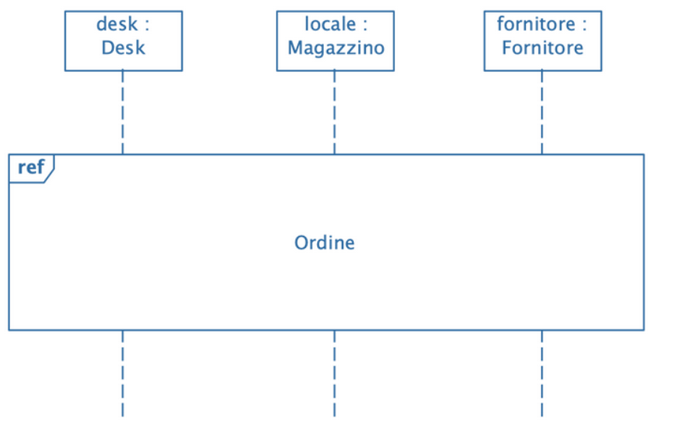
\includegraphics[scale=.4]{ref}
\end{center}

\subsection{Gate}
Un gate è un punto di ingresso o di uscita sul bordo di un diagramma o di un frame. Consente la spedizione e la ricezione di messaggi ed è identificato da un nome.
\begin{center}
	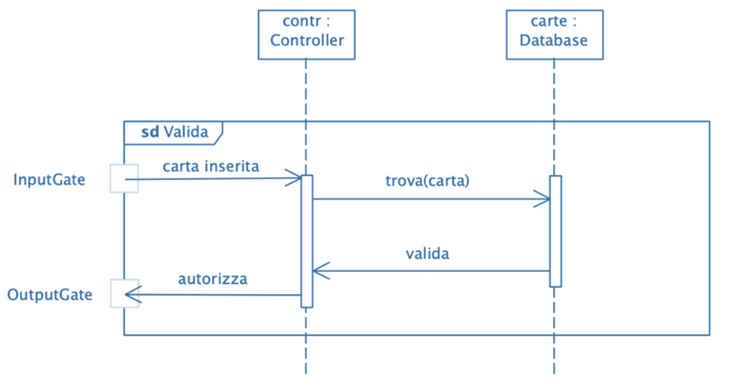
\includegraphics[scale=.4]{gate}
\end{center}

\subsection{Vincoli di durata}
Sono espressi tra parentesi graffe e consentono di specificare:
\begin{itemize}
	\item \textbf{quando} avviene un evento, tramite \textbf{at}(orario) o \textbf{now}
	\item \textbf{quanto} tempo tra due eventi, che può essere un numero effettivo o un range (min, max)
\end{itemize}
\begin{center}
	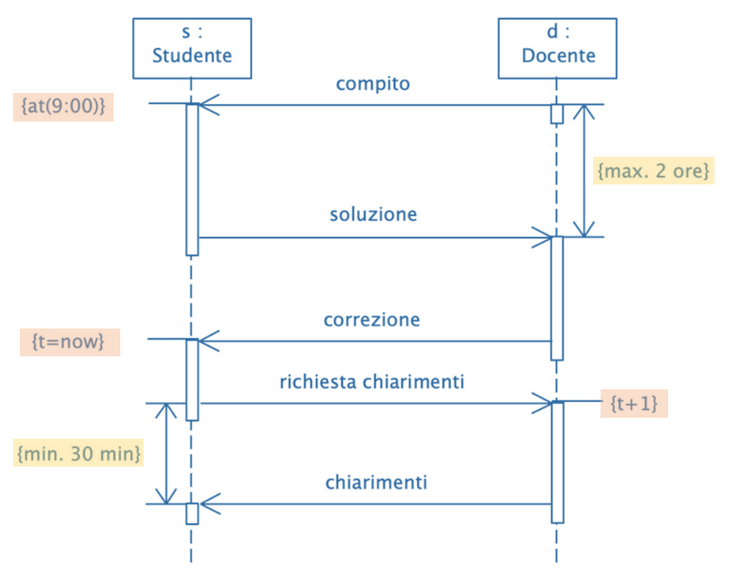
\includegraphics[scale=.4]{vincoli}
\end{center}
	% !TeX spellcheck = it_IT
\newpage
\section{Principi di progettazione}
Le tecniche di progettazione e le good practice mirano a produrre un sistema che realizzi \textbf{requisiti funzionali} e di \textbf{qualità}, mantenendolo facilmente \textbf{manutenibile} e \textbf{riusabile}.
\subsection{Principi generali}
\subsubsection{Information hiding}
Consiste nella separazione tra l'\textbf{interfaccia} visibile e il \textbf{corpo}, ovvero l'implementazione che è privata e/o nascosta. I componenti o i moduli sono come \textbf{black box} che forniscono e richiedono funzionalità. Rendono nota all'esterno solo la loro \textbf{interfaccia} ma nascondono algoritmi e strutture dati usati internamente.\\
I vantaggi principali sono:
\begin{itemize}
	\item \textbf{Comprensibilità}: non servono i dettagli implementativi per usare una feature
	\item \textbf{Manutenibilità}: si può cambiare il corpo di un'unità senza cambiarne altre
	\item \textbf{Team work}: corpi di unità diverse possono essere sviluppate da team indipendenti
	\item \textbf{Sicurezza}: i dati di un'unità sono modificabili solo internamente
\end{itemize}

\begin{observation}[Incapsulamento]
	L'incapsulamento è diverso dall'information hiding: il primo rappresenta la capacità degli oggetti di mantenere al loro interno attributi e metodi ed è una proprietà dei linguaggi di programmazione. Permette, \textit{senza garantire}, l'information hiding tramite i costrutti \textit{public} e \textit{private}
\end{observation}

Lo standard de-facto per l'accesso agli attributi privati, che quindi ne nasconde la rappresentazione, è tramite un'interfaccia di getter e setter:
\begin{itemize}
	\item \textbf{getter}: restituisce un attributo come valore e senza cambiare lo stato dell'oggetto
	\item \textbf{setter}: modifica lo stato dell'oggetto cambiando il valore dell'attributo
\end{itemize}

\subsubsection{Astrazione}
Il principio di astrazione si applica a:
\begin{itemize}
	\item \textbf{Controllo}: una procedura è vista come modulo di astrazione del flusso di controllo, nascondendo l'algoritmo utilizzato. Sono organizzate in classi di moduli e costituiscono la libreria.
	\item \textbf{Dati}: la struttura dati, che regolamenta accesso e modifica, è astratta, garantendo un'interfaccia stabile indipendentemente dal cambio di implementazione. Non sono puramente funzionali in quanto le operazioni offerte possono cambiare lo stato.
\end{itemize}

\subsubsection{Coesione}
La coesione è quanto strettamente correlate sono le funzionalità offerte da un modulo o da una componente. Funzionalità vicine devono stare nella stessa unità e un sistema è coeso se tutti gli elementi di ogni unità sono strettamente collegati. Esistono diversi tipi di coesione:
\begin{itemize}
	\item \textbf{Funzionale}: gli elementi collaborano per realizzare una funzionalità
	\item \textbf{Temporale}: gli elementi sono azioni che devono essere eseguite in uno stesso arco di tempo (difficilmente coese e riutilizzabili)
	\item \textbf{Logica}: gli elementi sono correlati logicamente ma non funzionalmente (e.g. raccolta dati, analisi e generazione dei report). Possono essere operazioni correlate ma funzioni significativamente diverse o operazioni debolmente connesse e difficilmente riutilizzabili
	\item \textbf{Accidentale}: gli elementi non sono correlati ma sono piazzati assieme
\end{itemize}

\subsubsection{Disaccoppiamento}
Indica quanto sono slegate le unità di progettazione in termini di dipendenze funzionali o messaggi. In un sistema molto accoppiato (\textbf{high coupling}) le modifiche alle varie unità impattano anche le altre a distanza, rendendo difficile la manutenzione. In quelli poco accoppiati (\textbf{low coupling}) l'impatto delle modifiche è limitato.

\begin{observation}
	Un alto grado di coesione contribuisce a ridurre il grado di accoppiamento.
\end{observation}

\subsection{Collezione di principi}
\subsubsection{SOLID}
SOLID include cinque principi di base per progettazione e sviluppo object oriented.
\begin{wrapfigure}[5]{r}{3.5cm}
	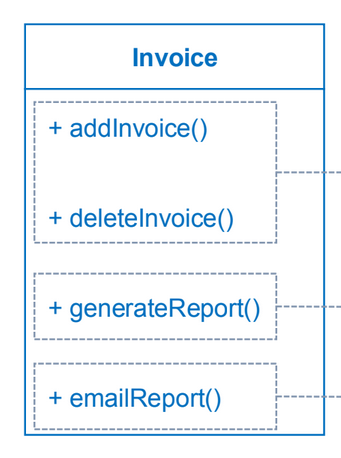
\includegraphics[width=3.5cm]{singleresp}
\end{wrapfigure}
\paragraph{Single Responsibility} Una classe o metodo deve avere un solo motivo per cambiare: un cambiamento deve impattare solo la classe che realizza quella funzionalità, se ci sono più motivi vanno create più classi. Deve quindi essere \textbf{funzionalmente coesa}.\\
Le eccezioni a questa regola sono:
\begin{itemize}
	\item La separazione di una classe introdurrebbe complessità non necessaria
	\item Un motivo di cambiamento è tale se è una reale possibilità di \\cambiamento nel sistema
\end{itemize}

\paragraph{Open Closed} Le entità software devono essere aperte per estensione ma chiuse per modifiche. Se i requisiti cambiano si deve estendere il comportamento aggiungendo nuovo codice, senza cambiare quello esistente e funzionante. Si può implementare tramite classi \textbf{astratte} e \textbf{concrete}, \textbf{delega} e \textbf{plugin}.

\paragraph{Liskov Substitution}
Deriva dal principio di sostituzione di Barbara Liskov.
\begin{definition}[Principio di sostituzione]
	Dato $S$ \textbf{sottotipo} di $T$, $o_s$ e $o_t$ oggetti di tipo rispettivamente $S$ e $T$ e $P$ un programma definito in termini di $T$. Se $o_s$ è usato al posto di $o_t$, il comportamento di $P$ è immutato. 
\end{definition}
\begin{center}
	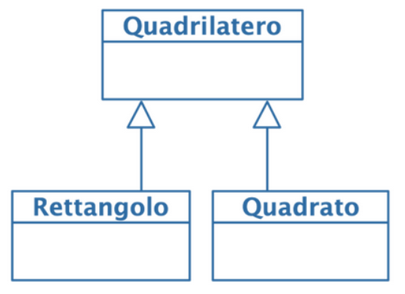
\includegraphics[scale=.4]{subst}
\end{center}

\paragraph{Interface Segregation} Le interfacce devono essere a \textbf{grana fine} e \textbf{specifiche} per ogni cliente: i client non devono dipendere da interfacce che non usano e si devono mettere solo i metodi utilizzati.
\begin{example}
	Ad esempio un lavoratore lavora e mangia. Può essere umano o robot ma quest'ultimo non può mangiare. Conviene quindi separare l'interfaccia del lavoratore da quello del mangiatore e il robot implementerà solo la prima.
\end{example}

\paragraph{Dependency Inversion} Si deve programmare per l'interfaccia e non per l'implementazione: i moduli di alto livello non devono dipendere da quelli di basso livello ma devono entrambi dipendere da \textbf{astrazioni} che a loro volta non devono dipendere dai dettagli.

\begin{example}
	Dati dei moduli per leggere, scrivere e copiare, è necessario che questi non dipendano, ad esempio, dal mezzo su cui eseguire le operazioni. Potrebbero essere implementate per la lettura da tastiera e scrittura su schermo oppure lettura da tastiera e scrittura su disco.
\end{example}

\subparagraph{Dependency Injection} È una forma di inversione delle dipendenze dove il cliente non sa come costruire i servizi che vuole chiamare ma delega ad un \textbf{iniettore}, che poi a sua volta passa al client i servizi. È quindi sufficiente sapere solo le interfacce dei servizi che definiscono come il client può usarli e in questo modo le responsabilità di costruzione e di utilizzo sono separate.

\subsubsection{GRASP}
Questa famiglia di principi di progettazione si compone di: \textbf{General Responsibility Assignment Software Patterns}. La progettazione è guidata dai \textbf{casi d'uso} che vengono realizzati in termini di oggetti collaborativi utilizzando diagrammi e pattern e assegnando responsabilità alle classi.\\

In particolare le \textbf{responsabilità} sono obblighi che un oggetto ha, definiti in termini di comportamento, e legate al dominio del problema. Possono essere di due tipi:
\begin{itemize}
	\item \textbf{Fare}: fare qualcosa (e.g. creare un oggetto o fare un calcolo) o iniziare, controllare e coordinare le azioni di altri oggetti
	\item \textbf{Conoscere}: conoscere i dati privati, gli oggetti correlati, i dati che possono derivare o calcolare. Generalmente si deducono dal modello di dominio.
\end{itemize}

\begin{observation}
	Una responsabilità non è un metodo: questi ultimi sono implementati per soddisfare le prime e la traduzione da responsabilità a metodi dipende dalla \textbf{granularità} della prima.
\end{observation}

\subsection{Delega}
L'ereditarietà presenta alcuni problemi: obbliga ad ereditare tutti i metodi anche se non rilevanti o non adatti e rende la sottoclasse strettamente legata all'implementazione della superclasse. La delega, al contrario, rende esplicito l'utilizzo parziale e consente di \textbf{controllare quanti e quali} metodi la classe delegata usa. Il costo è rappresentato dai metodi di delega aggiuntivi.\\

La delega riduce leggermente le \textbf{prestazioni} per l'invocazione di un altro oggetto rispetto all'uso di un metodo ereditato. Inoltre non può essere usata con classi astratte e non impone una struttura al progetto.

\subsection{Qualità del software}
\subsubsection{Functional suitability}
Il grado con cui un prodotto o un sistema fornisce funzionalità che soddisfino le richieste esplicite ed implicite quanto usato sotto certe condizioni. Si divide in:
\begin{itemize}
	\item \textbf{Functional completeness}: quando le funzionalità offerte coprono i task specificati e gli obiettivi degli utenti considerati
	\item \textbf{Functional correctness}: quanto siano accurati i risultati forniti agli utenti considerati
	\item \textbf{Functional appropriatness}: quanto le funzionalità offerte facilitano il raggiungimento del task e gli obiettivi considerati
\end{itemize}

\subsubsection{Performance efficiency}
Il grado con cui un sistema esegue le sue funzioni nella quantità di tempo specificata e con determinati parametri di output assieme alla sua efficienza nell'uso delle risorse date determinate condizioni. Si divide in:
\begin{itemize}
	\item \textbf{Time behaviour}: quanto vengono rispettati i requisiti in termine di \textit{response time} e \textit{throughput}
	\item \textbf{Resource utilization}: quanto vengono rispettati i requisiti  in termini di \textit{quantità} e \textit{tipologia} di risorse computazionali utilizzate
	\item \textbf{Capacity}: quanto vengono rispettati i requisiti in termini di capacità (limiti massimi)
\end{itemize}

\subsubsection{Compatibility}
Il grado con cui un sistema scambia informazioni con altri ed esegue funzioni mentre condivide lo stesso ambiente comune e le stesse risorse. Si divide in:
\begin{itemize}
	\item \textbf{Co-existance}: quanto il sistema rimane efficiente mentre condivide ambiente e risorse
	\item \textbf{Interoperability}: quanto il sistema riesce a scambiare informazioni con altri e sfruttare quelle ricevute
\end{itemize}

\subsubsection{Interaction capability}
Il grado con cui un sistema può interagire con utenti specifici per scambiare informazioni nell'interfaccia utente per completare task in diversi contesti. Si divide in:
\begin{itemize}
	\item \textbf{Appropriatness recognizability}: quanto gli utenti riconoscono se il sistema è appropriato
	\item \textbf{Learnability}: quanto le funzionalità sono apprendibili da un utente in un certo lasso di tempo
	\item \textbf{Operability}: quanto sia facile operare e controllare il sistema
	\item \textbf{User error protection}: quanto il sistema prevenga errori operativi
	\item \textbf{User engagement}: quanto \textit{engaging} sia il sistema
	\item \textbf{Inclusivity}: quanto il sistema può essere utilizzato da utenti con background diversi
	\item \textbf{User assistance}: quanto il sistema può essere usato da utenti diversi per gli stessi task
	\item \textbf{Self-descriptiveness}: quanto bene sono presentate le informazioni e le funzionalità per rendere ovvio l'utilizzo del sistema
\end{itemize}

\subsubsection{Reliability}
Il grado con cui un sistema esegua determinate funzioni in determinate condizioni per un certo periodo di tempo. Si divide in:
\begin{itemize}
	\item \textbf{Faultlessness}: quanto il sistema funziona senza fallimenti
	\item \textbf{Availability}: quanto il sistema sia operativo ed accessibile quando richiesto
	\item \textbf{Fault tolerance}: quanto il sistema riesca a ripristinare lo stato desiderato in caso di fallimento
\end{itemize}

\subsubsection{Security}
Il grado con cui un sistema riesce a difendersi da attacchi e proteggere le informazioni e i dati. Si divide in:
\begin{itemize}
	\item \textbf{Confidentiality}: quanto il sistema assicura che i dati siano accessibili solo a persone autorizzate
	\item \textbf{Integrity}: quanto il sistema assicura che lo stato del sistema e i dati siano protetti da modifiche non autorizzate
	\item \textbf{Non-repudiation}: quanto sia dimostrabile che azioni ed eventi abbiano avuto luogo
	\item \textbf{Accountability}: quanto sono tracciabili le azioni di una entità
	\item \textbf{Authenticity}: quanto è dimostrabile che l'identità di un soggetto o risorsa sia effettivamente quella
	\item \textbf{Resistance}: quanto il sistema è resistente da attacchi di malintenzionati
\end{itemize}

\subsubsection{Maintainability}
Il grado di efficacia ed efficienza con cui un sistema può essere modificato per migliorarlo, correggerlo o adattarlo a cambi dell'ambiente e dei requisiti. Si divide in:
\begin{itemize}
	\item \textbf{Modularity}: quanto poco i cambiamenti di un modulo di un sistema impattano sugli altri
	\item \textbf{Reusability}: quanto è riusabile il sistema e le sue parti
	\item \textbf{Analyzabilty}: quanto è facile analizzare l'impatto di un eventuale cambiamento, diagnosticare le cause di eventuali problemi o identificare le parti da modificare
	\item \textbf{Modifiability}: quanto sia modificabile il sistema senza degradarne le qualità
	\item \textbf{Testability}: quanto sia facile determinare i criteri di test e testare effettivamente il sistema
\end{itemize}

\subsubsection{Flexibility}
Il grado con cui un prodotto può essere adattato ai cambiamenti dei requisiti, del contesto o dell'ambiente.
\begin{itemize}
	\item \textbf{Adaptability}: quanto il sistema è adattabile a cambiamenti HW e SW degli ambienti di esecuzione
	\item \textbf{Scalability}: quanto bene il sistema gestisce i cambiamenti di workload e variability
	\item \textbf{Installability}: quanto efficientemente il sistema può essere installato o disinstallato
	\item \textbf{Replaceability}: quanto il sistema può sostituirne un altro sviluppato per gli stessi scopi
\end{itemize}

\subsubsection{Safety}
Il grado con cui un prodotto evita stati in cui la vita umana, la salute o gli oggetti siano messi in pericolo.
\begin{itemize}
	\item \textbf{Operational constraint}: quanto il sistema è vincolato a rimanere nei parametri di sicurezza
	\item \textbf{Risk identification}: quanto eventuali rischi di sicurezza sono identificati
	\item \textbf{Fail safe}: quanto in caso di fallimenti o pericoli il sistema riesca ad agire in safe mode
	\item \textbf{Hazard warning}: quanto il sistema fornisca avvisi su rischi inaccettabili per gli operatori in modo che essi possano reagire spontaneamente
	\item \textbf{Safe integration}: quanto il sistema riesca a mantenere la \textit{safety} se integrato con altri sistemi
\end{itemize}

\newpage
\subsection{Qualità delle implementazioni}
\subsubsection{Client-Server 2-N tier}
\begin{table}[!h]
	\centering
	\begin{tabular}{|c|p{10cm}|}
		\hline
		\textbf{Disponibilità} & I server di ogni tier possono essere replicati quindi in caso di fallimento il problema sarebbe minimo.\\
		\hline
		\textbf{Fault tolerance}&Se un client sta comunicando con un server che fallisce, la richiesta viene reindirizzata ad un server replicato in maniera trasparente. \\
		\hline
		\textbf{Modificabilità} & Il disaccoppiamento e la coesione di questa architettura favoriscono la modificabilità.\\
		\hline
		\textbf{Performance} & Buone performance ma bisogna tenere d'occhio il numero di threads, la velocità delle comunicazioni e il volume dei dati scambiato.\\
		\hline
		\textbf{Scalabilità} & Basta replicare i server di ogni tier. Unico bottleneck potrebbe essere la base di dati in comune.\\
		\hline
	\end{tabular}
\end{table}

\subsubsection{Pipes and filters}
\begin{table}[!h]
	\centering
	\begin{tabular}{|c|p{10cm}|}
		\hline
		\textbf{Disponibilità} & Avendo componenti e possibilità di connetterli sufficienti a formare una catena.\\
		\hline
		\textbf{Fault tolerance}&Occorre riparare una catena interrotta usando componenti replica. \\
		\hline
		\textbf{Modificabilità} & Presente se le modifiche interessano una o poche componenti.\\
		\hline
		\textbf{Performance} & Dipende dalla capacità del canale di comunicazione e dalla performance del filtro più lento.\\
		\hline
		\textbf{Scalabilità} & Ok.\\
		\hline
	\end{tabular}
\end{table}

\subsubsection{Publish-Subscribe}
\begin{table}[!h]
	\centering
	\begin{tabular}{|c|p{10cm}|}
		\hline
		\textbf{Disponibilità} & Si possono creare cluster di dispatcher.\\
		\hline
		\textbf{Fault tolerance}&Si crea un dispatcher replica. \\
		\hline
		\textbf{Modificabilità} & Si possono aggiungere publisher e subscriber ponendo attenzione al formato dei messaggi.\\
		\hline
		\textbf{Performance} & Ok ma con un compromesso tra velocità e requisiti tipo affidabilità e/o sicurezza.\\
		\hline
		\textbf{Scalabilità} & Con un cluster si può gestire un volume molto elevato di messaggi.\\
		\hline
	\end{tabular}
\end{table}

\subsubsection{P2P}
\begin{table}[!h]
	\centering
	\begin{tabular}{|c|p{10cm}|}
		\hline
		\textbf{Disponibilità} & Dipende dal numero di nodi, si assume di si.\\
		\hline
		\textbf{Fault tolerance}&Gratis. \\
		\hline
		\textbf{Modificabilità} & Si se si è interessati solo alla parte di comunicazione.\\
		\hline
		\textbf{Performance} & Dipende dal numero di nodi, dalla rete e dagli algoritmi.\\
		\hline
		\textbf{Scalabilità} & Gratis.\\
		\hline
	\end{tabular}
\end{table}
	% !TeX spellcheck = it_IT
\newpage
\section{Design pattern}
La progettazione non è solo un processo creativo. Il progettista può infatti seguire una serie di regole pratiche, appunto i design patterns, che descrivono il cuore della soluzione ad un problema frequente in modo che questa possa essere riutilizzata tante volte.\\

Nel software in particolare i pattern (soluzioni create in passato) vengono utilizzati per avere una maggiore \textbf{produttività} e rendere i progetti più \textbf{flessibili}.\\

\subsection{Gang of Four}
\subsubsection{Classificazione}
Nell'ambito della \textbf{progettazione di dettaglio}, \textbf{GoF} i pattern sono classificati in base al loro scopo e divisi in tre categorie:
\begin{itemize}
	\item \textbf{Creazionali}: riguardano la creazione di oggetti
	\begin{itemize}
		\item \textit{Abstract Factory}
		\item \textit{Builder}
		\item \textit{Factory Method}
		\item \textit{Prototype}
		\item \textit{Singleton}
	\end{itemize}
	\item \textbf{Strutturali}: riguardano la composizione di classi ed oggetti
	\begin{itemize}
		\item \textit{Adapter}
		\item \textit{Bridge}
		\item \textit{Composite}
		\item \textit{Decorator}
		\item \textit{Façade}
		\item \textit{Flyweight}
		\item \textit{Proxy}
	\end{itemize}
	\item \textbf{Comportamentali}: riguardano le interazioni tra classi ed oggetti e la suddivisione delle loro responsabilità
	\begin{itemize}
		\item \textit{Chain of responsibility}
		\item \textit{Command}
		\item \textit{Interpreter}
		\item \textit{Iterator}
		\item \textit{Mediator}
		\item \textit{Memento}
		\item \textit{Observer}
		\item \textit{State}
		\item \textit{Strategy}
		\item \textit{Template}
		\item \textit{Visitor}
	\end{itemize}
\end{itemize}

\newpage
\subsubsection{Template}
Un buon template per un pattern secondo GoF è il seguente:
\begin{table}[!h]
	\centering
	\begin{tabular}{|c|c|}
		\hline
		\textbf{Pattern name and classification} & Un nome breve e conciso per un pattern ed il suo tipo \\
		\hline
		\textbf{Intent} & Una breve frase su cosa fa il pattern \\
		\hline
		\textbf{Also known as} & Altri nomi \\
		\hline
		\textbf{Motivation} & Uno scenario che mostri perché è utile \\
		\hline
		\textbf{Applicability} & Situazioni dove può essere usato \\
		\hline
		\textbf{Structure} & Rappresentazione grafica \\
		\hline
		\textbf{Participants} & Le classi e gli oggetti che lo compongono\\
		\hline
		\textbf{Collaborations} & Come i partecipanti rispettano le loro responsabilità \\
		\hline
		\textbf{Consequences} & Pro e contro \\
		\hline
		\textbf{Implementation} & Suggerimenti e tecniche per l'implementazione \\
		\hline
		\textbf{Sample code} & Frammenti di codice per una semplice implementazione \\
		\hline
		\textbf{Known users} & Esempi in sistemi reali \\
		\hline
		\textbf{Related patterns} & Altri pattern strettamente correlati \\
		\hline
	\end{tabular}
\end{table}

\subsubsection{Notazione}
GoF utilizza come notazione la \textbf{Object Modeling Technique}.
\begin{center}
	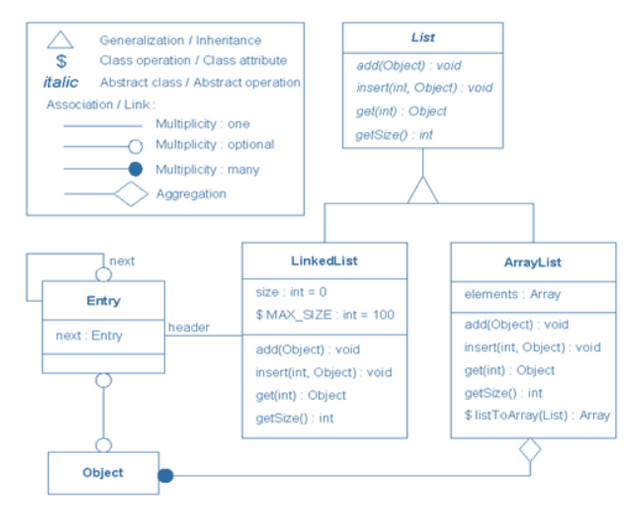
\includegraphics[scale=.5]{gof}
\end{center}

\newpage
\subsection{Strategy}
Lo strategy design pattern prevede di definire una famiglia di algoritmi, incapsularli separatamente e renderli intercambiabili. Questo permette ad essi di cambiare indipendentemente dai clienti che li usano.\\
Un programma potrebbe dover fornire più \textbf{varianti} di un algoritmo: le variazioni vengono incapsulate in classi separate mentre il metodo per l'accesso ad esse rimane uniforme.\\
Lo strategy design pattern si compone di tre partecipanti:
\begin{itemize}
	\item \textbf{Strategy}: definisce un'interfaccia comune per gli algoritmi
	\item \textbf{ConcreteStrategy}: ogni strategia concreta implementa un algoritmo
	\item \textbf{Context}: contiene un riferimento ad un oggetto \textit{strategy} e può definire un'interfaccia che le consente di accedere ai dati di interesse invece di doverli passare come argomenti
\end{itemize}

\begin{example}[MyArray]
	La classe \textit{MyArray} rappresenta un vettore di numeri. Uno dei suoi metodi lo stampa in due possibili formati che potrebbero però cambiare in futuro:
	\begin{itemize}
		\item \textit{MathFormat}, e.g. $\{12,-7,3,\ldots\}$
		\item \textit{StandardFormat}, e.g. ar[0]=12, ar[1]=-7, ar[2]=3,...
	\end{itemize}
	Usiamo lo strategy design pattern per isolare l'algoritmo di formattazione in modo che possa variare indipendentemente dal resto della classe.
	\begin{center}
		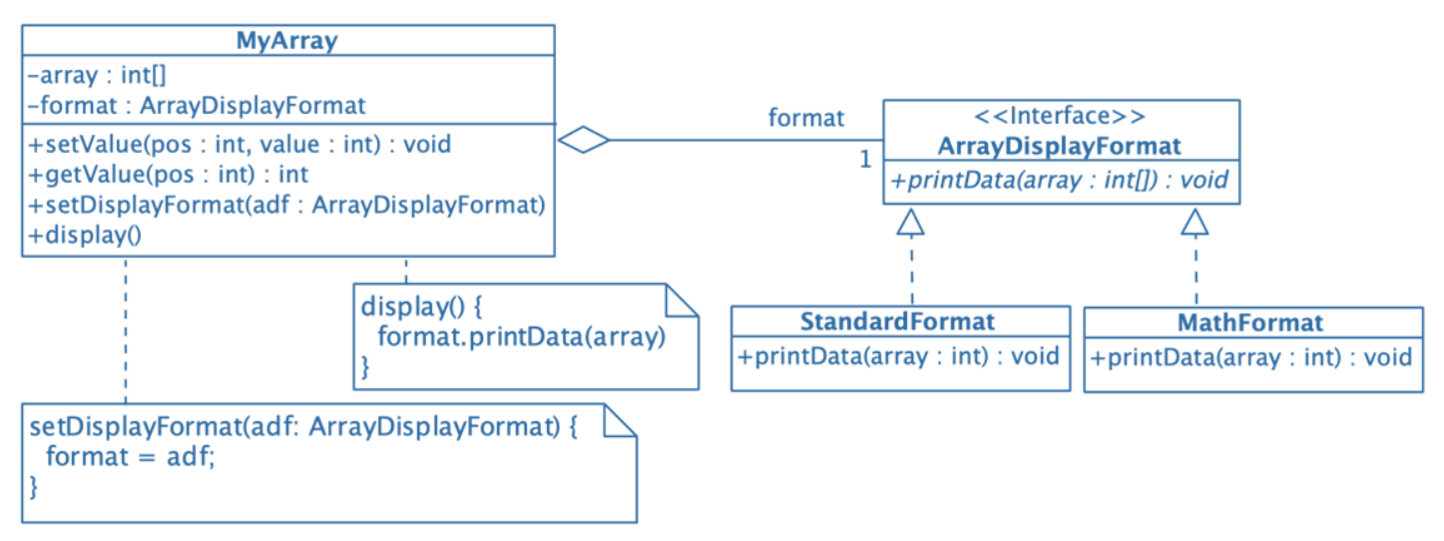
\includegraphics[scale=.3]{myarray}
	\end{center}
	La \textit{strategy} è \textit{ArrayDisplayFormat}, le \textit{ConcreteStrategy} sono \textit{StandardFormat} e \textit{MathFormat} e il \textit{Context} è \textit{MyArray}.
\end{example}

\subsubsection{Conclusioni}
Lo strategy pattern è utile nei seguenti casi:
\begin{itemize}
	\item Più classi correlate differiscono solo nel \textbf{comportamento}
	\item Servono più \textbf{varianti} diverse di un algoritmo
	\item Un algoritmo usa dei dati che i clienti non conoscono
	\item Evitare di esporre strutture dati complesse e algorithm-specific
\end{itemize}

\begin{note}
	Quando una classe definisce molti comportamenti che appaiono come alternative in costrutti condizionali, può essere utile trasformare i branch in classi ottenute con lo strategy pattern.
\end{note}

Il \textbf{costo} dello strategy pattern è di incrementare il numero di oggetti presenti in un'implementazione e la necessità di garantire che le implementazioni diverse rispettino la stessa interfaccia.

\begin{observation}[Dati diversi]
	Può capitare che strategie diverse usino dati diversi e che quindi in certe \textit{ConcreteStrategy} non tutti i dati vengano utilizzati. Per evitare l'inizializzazione di questi ultimi, si deve fare un \textbf{coupling} maggiore tra \textit{ConcreteStrategy} e \textit{Context}, dove le prime devono chiedere al secondo solo i dati necessari.
\end{observation}
\subsection{State}
Lo state design pattern è un \textbf{behavioural pattern}, ovvero che consente ad un oggetto di alterare il suo comportamento quando cambia lo stato interno. Si compone di tre partecipanti:
\begin{itemize}
	\item \textbf{Context}: definisce l'interfaccia di interesse per i client e mantiene un'istanza di \textit{ConcreteState} che definisce lo stato corrente
	\item \textbf{State}: incapsula il comportamento associato ad un particolare stato del \textit{Context}. Può anche essere una classe concreta con un'implementazione predefinita.
	\item \textbf{Concrete state}: sono sottoclassi dello stato che implementano il comportamento associato allo \textit{State} che rappresentano.
\end{itemize}
Vediamo i passaggi per implementare lo state pattern:
\begin{enumerate}
	\item Identificare o creare una classe (\textbf{Context}) che funga da macchina a stati dal punto di vista del cliente
	\item Creare una classe \textbf{State} che replichi i metodi dell'interfaccia della macchina a stati: ogni metodo richiederà un parametro aggiuntivo (un'istanza della classe di \textit{Context})
	\item Creare una \textbf{sottoclasse} di \textit{State} per ogni stato del dominio, ognuna delle quali sovrascrive solo i metodi che cambiano
	\item La classe di \textit{Context} mantiene lo \textbf{stato corrente}, che è un oggetto della classe di \textit{State}
	\item Le richieste dei client sono delegate dalla classe di \textit{Context} allo stato corrente, passando ad esse anche l'oggetto di \textit{Context}
	\item I metodi della classe \textit{State} modificano lo stato corrente
\end{enumerate}

\begin{example}[TCP]
	Un esempio è l'implementazione del protocollo TCP, che invia risposte diverse a seconda dello stato della connessione.
	\begin{center}
		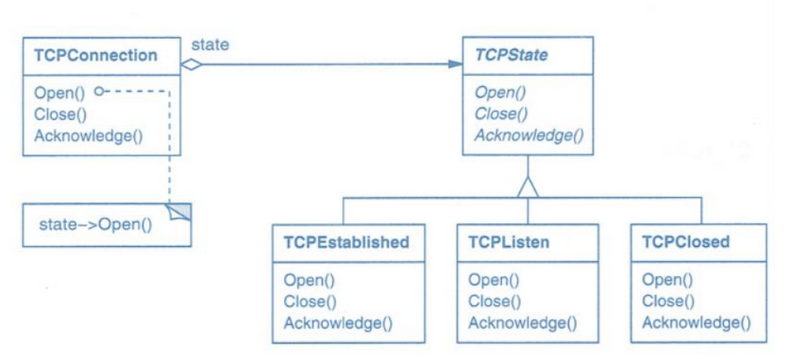
\includegraphics[scale=.4]{tcp}
	\end{center}
\end{example}

\subsubsection{Conclusioni}
Lo state pattern è utile nei seguenti casi:
\begin{itemize}
	\item Il \textbf{comportamento} di un oggetto dipende dal suo stato
	\item Le operazioni hanno \textbf{dichiarazioni condizionali complesse}, dove la scelta dipende dallo stato
\end{itemize}

\begin{observation}
	Il comportamento è suddiviso tra i possibili stati e ognuno è memorizzato in una classe.
\end{observation}
\begin{observation}
	Lo stato corrente è memorizzato in un'unica posizione e le transizioni di stato sono esplicite.
\end{observation}
\begin{observation}
	La classe \textit{State} può implementare parte del comportamento se è in comune o di default. Inoltre i suoi oggetti possono essere condivisi quando non hanno variabili di istanza.
\end{observation}

\subsection{Factory}
Le factory sono dei pattern di tipo \textbf{creazionale}: astraggono il processo di instanziazione degli oggetti nascondendo l'effettiva creazione e rendendo il sistema indipendente da ciò.\\
Una classe \textit{factory} ha il solo compito di creare e restituire istanze di altre classi.

\begin{observation}[New]
	Il comando \textit{new} viola il principio \textit{code to an interface} in quanto assegniamo ad una variabile un oggetto ottenuto da una classe concreta. Questa dipende da ogni classe riferita al suo interno e deve essere aggiornata e ricompilata se cambiano le classi riferite, violando i principi \textit{open-closed} e \textit{information hiding}.
\end{observation}

\subsubsection{Simple factory}
Detto anche ConcreteFactory, non appartiene alla Gang of Four ed è una semplificazione molto diffusa di \textit{Abstract Factory}. Consiste nel delegare ad un oggetto \textbf{factory} la creazione separandola dalle altre funzionalità.
\begin{center}
	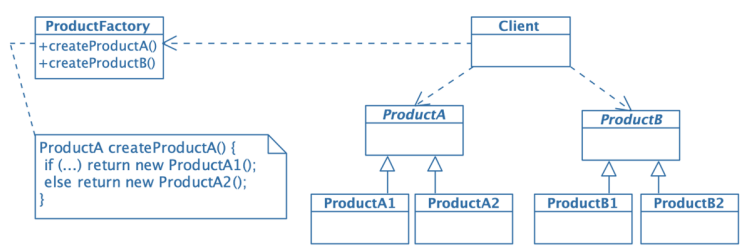
\includegraphics[scale=.5]{simplefactory}
\end{center}

\subsubsection{Factory method}
Il factory method delega alle sottoclassi la decisione di quali classi istanziare. Si compone di quattro partecipanti:
\begin{itemize}
	\item \textbf{Creator} (astratto o concreto): dichiara il \textbf{factory method} che viene usato da altri metodi. Questo, se crea tipi diversi di prodotti, deve avere un parametro.
	\item \textbf{ConcreteCreator}: sovrascrive il \textit{factory method} per restituire un istanza del \textit{ConcreteProduct}
	\item \textbf{ConcreteProduct}: implementa l'interfaccia di \textit{Product}
	\item \textbf{Product}: definisce l'interfaccia per il tipo di oggetti che sono creati dal \textit{factory method}
\end{itemize}
\begin{center}
	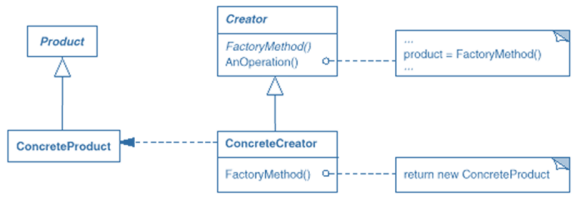
\includegraphics[scale=.6]{factorymethod}
\end{center}

Il factory method pattern permette di disaccoppiare una classe dalle classi degli oggetti che crea e utilizza e delega alle sottoclassi la specifica degli oggetti da creare. Rende il codice più \textbf{flessibile} e \textbf{riusabile} e implementa il principio di \textit{code to an interface} (la classe si basa sull'interfaccia di \textit{Product} e può funzionare con qualunque \textit{ConcreteProduct} che la supporti).\\

Lo \textbf{svantaggio} principale è la necessità di estendere la classe \textit{Creator} solo per istanziare un particolare \textit{ConcreteProduct}.

\subsubsection{Abstract factory}
L'abstract factory delega ad altre classi la decisione di quali classi istanziare. Definisce un'interfaccia per creare famiglie di oggetti correlati e dipendenti fra loro senza specificare le classi concrete.\\
A differenza del \textit{factory method}, l'abstract delega ad altri oggetti l'istanziazione tramite la \textbf{composizione}. Questi altri oggetti spesso usano il \textit{factory method}.
\begin{center}
	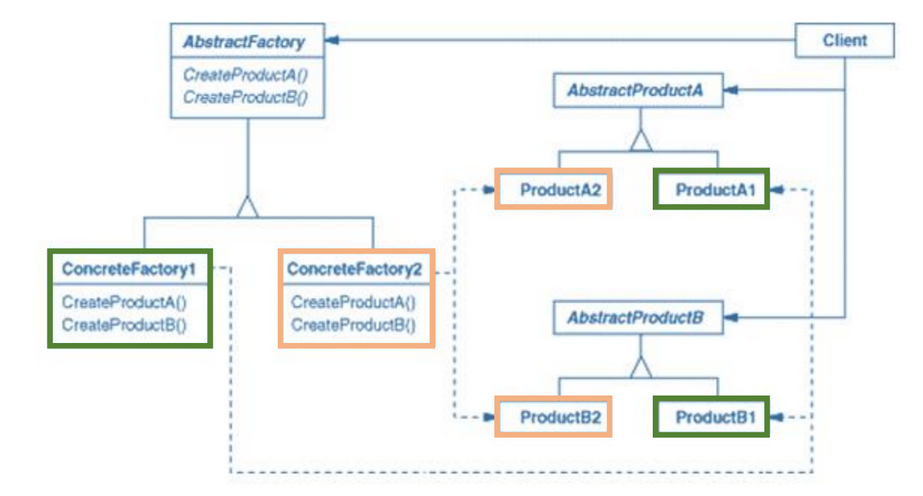
\includegraphics[scale=.3]{abstractfactory}
\end{center}

\subsubsection{Pure fabrication}
Si tratta di un pattern \textbf{GRASP} che assegna responsabilità fortemente correlate ad una \textbf{classe artificiale} che non rappresenta niente nel dominio del problema (è introdotta solo per convenienza). Implementa il \textbf{behavioural decomposition} con l'obiettivo di supportare \textit{high coesion}, \textit{low coupling} e \textit{riuso}.

\subsection{Singleton}
Il singleton pattern garantisce che una classe abbia \textbf{una sola istanza} fornendo un punto di accesso globale ad essa. 
\begin{note}
	Nonostante la necessità di avere oggetti unici sia abbastanza comune, in quanto spesso gran parte degli oggetti in un'applicazione hanno un'unica responsabilità assegnata, le classi singleton sono rare.
\end{note}
\noindent Per costruirlo:
\begin{enumerate}
	\item Si rende privato il costruttore della classe
	\item Si aggiunge un oggetto statico privato che conterrà l'unica istanza disponibile
	\item Si rende l'unica istanza disponibile accessibile solo tramite un metodo statico
\end{enumerate}

\begin{wrapfigure}[5]{r}{4cm}
	\vspace{-.5cm}
	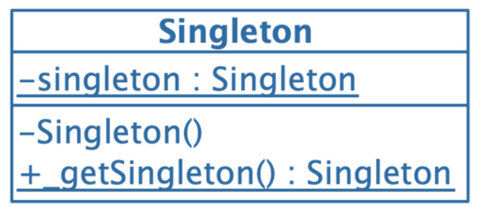
\includegraphics[width=4cm]{singleton}
\end{wrapfigure}
\subsubsection{Inizializzazione lazy} A volte non si potrebbero avere \textbf{sufficienti informazioni} per l'istanziazione del singleton statico oppure potrebbe essere molto \textbf{resource intensive}. In questo caso è meglio aspettare per eseguire l'inizializzazione.

\subsubsection{Multithread} Thread diversi potrebbero inizializzare più istanze del singleton quasi simultaneamente. Ci sono tre possibili soluzioni:
\begin{itemize}
	\item \textbf{Inizializzazione eager} invece di quella \textit{lazy}, spreca risorse
	\item \textbf{Sincronizzazione} del metodo \textit{getInstance}, dichiarandolo come \textit{synchronized}, riduce le performance
	\item \textbf{Double-checked locking}: una variabile volatile garantisce che ogni thread acceda all'ultimo valore assegnatole e solo un thread alla volta può eseguire un blocco di codice synchronized.
\end{itemize}

\subsubsection{Sottoclassi}
Nel caso in cui una classe singleton venga estesa, per garantire che l'unica istanza sia istanza di una sottoclasse, facciamo in modo che ognuna di esse fornisca un metodo statico \textit{getIstance}. In questo modo i costruttori delle sottoclassi possono essere privati e quello del singleton sarà \textbf{protected}.

\subsection{Decorator}
Il pattern decorator aggiunge dinamicamente \textbf{responsabilità} ad un oggetto ed è un'alternativa flessibile all'ereditarietà per l'aggiunta di funzionalità a \textbf{runtime}. Il pattern si compone di:
\begin{itemize}
	\item \textbf{Component}: interfaccia degli oggetti decorati
	\item \textbf{ConcreteComponent}: oggetti decorabili con nuove responsabilità
	\item \textbf{Decorator}: interfaccia conforme a quella comune che mantiene un riferimento ad un oggetto di tipo \textit{Component} (che può essere o meno già decorato)
	\item \textbf{ConcreteDecorator}: aggiunge nuove responsabilità
\end{itemize}
\begin{center}
	\includegraphics[scale=.5]{decorator}
\end{center}
È più \textbf{semplice} rispetto all'ereditarietà multipla e garantisce più \textbf{flessibilità} di quella statica. Favorisce inoltre l'aggiunta incrementale di feature.\\
I contro principali è che se troppo complessi i decorator diventano \textbf{costosi} e quando ce ne sono tanti piccoli i sistemi diventano \textbf{complessi} da gestire. Inoltre è importante notare che \textit{Decorator} e \textit{Component} non sono identici e quindi quando usiamo questo pattern è meglio non affidarsi all'identità degli oggetti.

\subsection{Adapter}
Nell'ambito della programmazione l'adapter permette a due codici con interfacce diverse di essere collegati. Questo pattern quindi \textbf{converte} l'interfaccia di una classe in quella attesa dal cliente. Si compone di:
\begin{itemize}
	\item \textbf{Target}: definisce l'interfaccia application-specific usata da \textit{Client}
	\item \textbf{Client}: interagisce con oggetti conformi a \textit{Target}
	\item \textbf{Adaptee}: definisce un'interfaccia esistente da adattare
	\item \textbf{Adapter}: adatta l'interfaccia di \textit{Adaptee} per renderla conforme a quella \textit{Target}. Questo binding è realizzato con il meccanismo di \textbf{delega}.
\end{itemize}
\begin{center}
	\includegraphics[scale=.6]{adapter}
\end{center}
Gli adapter possono essere realizzati come \textbf{strategie}: se abbiamo diversi moduli che implementano la stessa funzionalità e abbiamo scritto degli adattatori per loro, abbiamo un insieme di adattatori che implementano la stessa interfaccia e quindi possiamo sostituire gli oggetti adattatori in fase di esecuzione.

\subsubsection{Façade}
Il pattern façade è della Gang of Four e realizza un adattatore che inoltra le richieste a più \textit{adaptee} simultaneamente.

\subsection{Proxy}
Il proxy fornisce un surrogato per un altro oggetto per controllarne l'accesso. A differenza dell'adapter, il proxy e l'oggetto originale hanno la stessa interfaccia e può eseguire pre e post processing.\\
\begin{figure}[!h]
	\hfill
	\subfigure[Proxy pattern]{\includegraphics[width=7cm]{proxy}}
	\hfill
	\subfigure[Dynamic model]{\includegraphics[width=7cm]{proxydyn}}
	
\end{figure}

\noindent Ne esistono diversi tipi:
\begin{itemize}
	\item \textbf{Remote}: permette l'acceso ad un oggetto remoto
	\item \textbf{Protection}: implementa un controllo sugli accessi
	\item \textbf{Cache}: mantiene coppie di tipo richiesta-risposta per alleggerire il carico sul server
	\item \textbf{Synchronization}: gestisce gli accessi concorrenti ad un servizio
	\item \textbf{Virtual}: si comporta come l'originale mentre questi viene costruito e poi passa le richieste a quest'ultimo. È utile per ritardare la creazione di un oggetto costoso, che viene quindi creato solo al momento necessario mentre il proxy fa da surrogato.
\end{itemize}

\subsubsection{Java RMI}
Il proxy è molto simile a Java RMI che si compone del \textbf{client helper} che fa da \textbf{stub} e dal \textbf{service helper} che fa da \textbf{skeleton}:
\begin{enumerate}
	\item Il client fa una ricerca nel registro RMI
	\item Il registro restituisce un oggetto \textit{stub}, ovvero il remote proxy del servizio
	\item Il client invoca lo \textit{stub} come se fosse il servizio
\end{enumerate}
\end{document}
